\documentclass[journal]{IEEEtran}
\usepackage[a5paper, margin=10mm, onecolumn]{geometry}
\usepackage{lmodern}
\usepackage{tfrupee}
\setlength{\headheight}{1cm}
\setlength{\headsep}{0mm}

\usepackage{gvv-book}
\usepackage{gvv}
\usepackage{cite}
\usepackage{amsmath,amssymb,amsfonts,amsthm}
\usepackage{algorithmic}
\usepackage{graphicx}
\usepackage{textcomp}
\usepackage{xcolor}
\usepackage{txfonts}
\usepackage{listings}
\usepackage{enumitem}
\usepackage{mathtools}
\usepackage{gensymb}
\usepackage{comment}
\usepackage[breaklinks=true]{hyperref}
\usepackage{tkz-euclide}
\usepackage{listings}
\def\inputGnumericTable{}
\usepackage[latin1]{inputenc}
\usepackage{color}
\usepackage{array}
\usepackage{longtable}
\usepackage{calc}
\usepackage{multirow}
\usepackage{hhline}
\usepackage{ifthen}
\usepackage{lscape}
\usepackage{xparse}

\bibliographystyle{IEEEtran}

\title{5.2.45}
\author{EE25BTECH11043 - Nishid Khandagre}

\begin{document}
\maketitle

\renewcommand{\thefigure}{\theenumi}
\renewcommand{\thetable}{\theenumi}

\numberwithin{equation}{enumi}
\numberwithin{figure}{enumi}

\textbf{Question}:\
Solve the system of linear equations:
\begin{align}
x + 2y &= 2 \\
2x + 3y &= 3
\end{align}

\textbf{Solution: }
We have:
\begin{align}
x+2y&=2 \\
2x+3y&=3
\end{align}

\begin{align}
\myvec{1&2\\2&3}\myvec{x\\y}&=\myvec{2\\3}
\end{align}

Write augmented matrix
\begin{align}
\myaugvec{2}
{1 & 2 & 2 \\
2 & 3 & 3}
\end{align}

Eliminate first column
$R_2 \to R_2 - 2R_1$
\begin{align}
\myaugvec{2}
{1 & 2 & 2 \\
0 & -1 & -1}
\end{align}

Then
$R_2 \to -R_2$
\begin{align}
\myaugvec{2}
{1 & 2 & 2 \\
0 & 1 & 1}
\end{align}

Then
$R_1 \to R_1 - 2R_2$
\begin{align}
\myaugvec{2}
{1 & 0 & 0 \\
0 & 1 & 1}
\end{align}

\begin{align}
\myvec{x\\y}&=\myvec{0\\1}
\end{align}

Therefore
\begin{align}
x = 0 \\
y = 1
\end{align}
\begin{figure}[H]
    \centering
    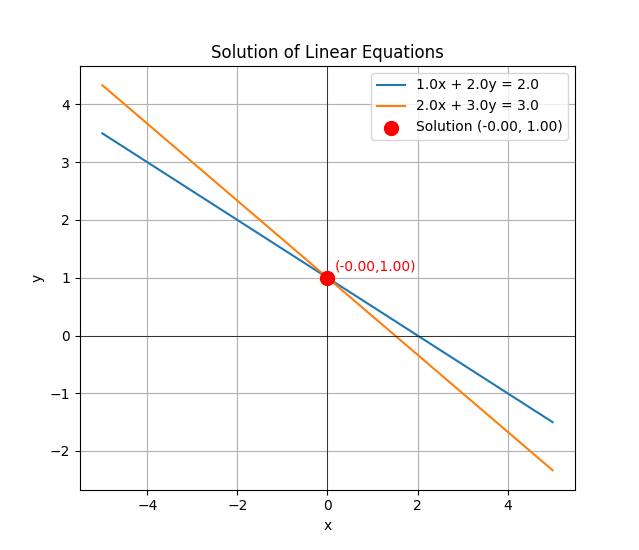
\includegraphics[width=0.8\columnwidth]{figs/fig1.png}
    \caption{}
    \label{fig:1}
\end{figure}



\end{document}
